	\chapter{Kravspecifikation}
	
	\section{Aktør kontekst diagram}
		På figur \ref{fig:AktorKontekst} ses aktør kontekst diagrammet for Rambøll Tilsyn. Diagrammet viser, hvilke aktør der interagerer med systemet.
	\begin{figure}[H]
		\centering
		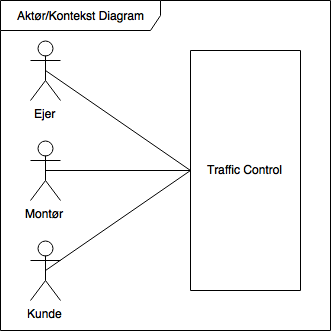
\includegraphics[width=0.6\linewidth]{Kravspecifikation/AktorDiagram}
		\caption{Aktør kontekst diagram for Rambøll Tilsyn}
		\label{fig:AktorKontekst}
	\end{figure}

	På venstre side af figur \ref{fig:AktorKontekst} ses brugeren som er den primære aktør af systemet. Brugeren benytter systemet, som på diagrammet bliver symboliseret som en blackbox. På højre side, ses de sekundære aktører. Disse aktører er dem som systemet bruger. Microsoft Office er en sekundær bruger, da systemet eksportere til Excel.
	
	\clearpage
	
\section{User stories diagram}
	Figur \ref{fig:Userstoriediagram} vises systemets User Stories diagram. Dette diagram viser den funktionalitet som systemet indeholder beskrevet gennem en række user stories.
	
	\begin{figure}[H]
		\centering
		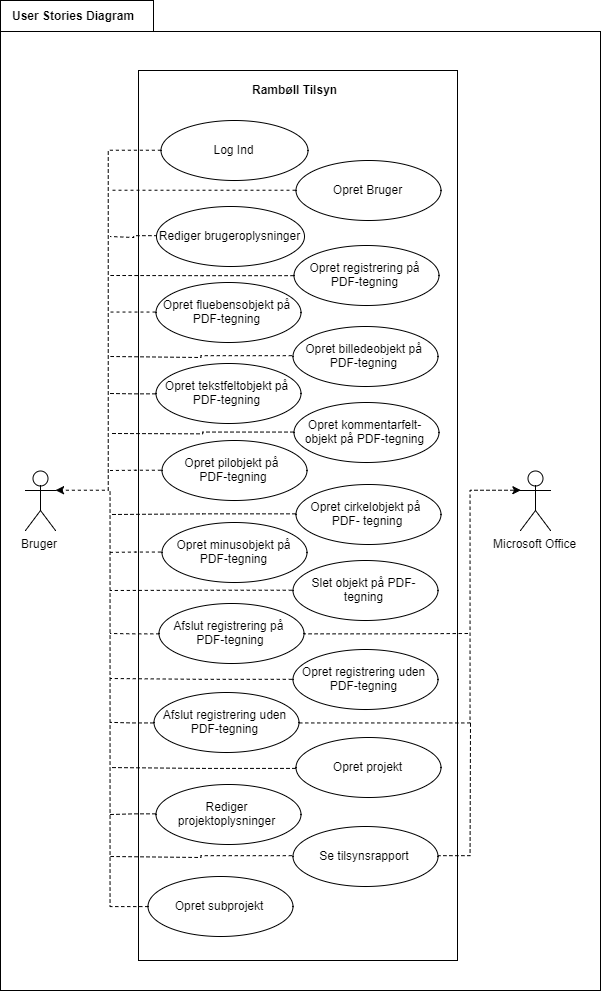
\includegraphics[width=0.6\linewidth]{Kravspecifikation/UserStorieDiagram}
		\caption{User stories diagram for Rambøll Tilsyn}
		\label{fig:Userstoriediagram}
	\end{figure}
	
	\clearpage
	
\section{Funktionelle krav} 
	Følgende er en kort beskrivelse af must user stories til Rambøll Tilsyn, som er fundet sammen med Rambøll ved hjælp af MoSCoW analyse. \cite{MoSCoW} For alle user stories fuldt beskrevet med Gherkin, se kravspecifikationen afsnit \ref{Krav-sec:UserStories}.

	\subsection*{Log-in (CRS-1)}
	Som bruger\\
	Ønsker jeg at kunne logge ind på applikationen\\
	For at kunne benytte applikationen
	
	\subsection*{Opret bruger (CRS-2)}
	Som ejer\\
	Ønsker jeg at kunne oprette bruger på applikationen\\
	For at kunne give en ny bruger adgang til systemet
	
	\subsection*{Opret en registrering på PDF tegning (CRS-4)}
	Som bruger\\
	Ønsker jeg at kunne oprette en registrering på PDF tegning\\
	For at have kunne lave en registrering på et givet projekt 
	
	\subsection*{Opret fluebens opbjekt på PDF tegning (CRS-5)}
	Som bruger \\
	Ønsker jeg at kunne oprette et fluebens opbjekt\\
	For kunne indikere at konstruktionen er godkendt 

	\subsection*{Opret billede opbjekt på PDF tegning (CRS-6)}
	Som bruger\\
	Ønsker jeg at kunne oprette et billede objekt\\
	For at kunne tage et billede og vedlægge som dokumentation 
	
	\subsection*{Opret tekstfelt opbjekt på PDF tegning (CRS-7)}
	Som bruger\\
	Ønsker jeg at kunne oprette et tekstfelt\\
	For at kunne skrive en kommentar til en del af konstruktionen 
	
	\subsection*{Opret minus opbjekt på PDF tegning (CRS-11)}
	Som bruger\\
	Ønsker jeg at kunne oprette et minus objekt\\
	For at kunne indikere at der er en fejl konstruktionen

	\subsection*{Slet opbjekt på PDF tegning (CRS-12)}
	Som bruger\\
	Ønsker jeg at kunne slette et objekt\\
	For at kunne fjerne objekter som enten er forkerte eller en fejl 

	\subsection*{Afslut registrering på PDF tegning (CRS-13)}
	Som bruger\\
	Ønsker jeg at kunne afslutte en registrering\\
	For at kunne se en liste over tilsyns registreringerne
	
	\subsection*{Opret projekt (CRS-16)}
	Som bruger\\
	Ønsker jeg at oprette et nyt projekt\\
	For at kunne oprette nye projekter løbende \\
	

\section{Ikke-funktionelle krav}
De ikke-funktionelle krav definere de tekniske krav som systemet skal indeholde. Disse krav beskriver egenskaber som ikke har indvirkning på systemets funktionelle krav. Dette kunne være antal brugere der benytter systemet samtidig eller hvordan brugerne skal have skrive og læse rettigheder. \\
Projektes ikke-funktionelle krav kan findes i afsnit \ref{Krav-sec:Ikkefunktionelle} i kravspecifikationen under bilag. \\


\section{Afgrænsning}
For at afgrænse projektet blev der holdt et møde med Rambøll, hvor de kunne komme med inputs til systemet. \\
Der blev lavet en MoSCoW analyse til at prioriterer funktionaliteten i systemet. Denne analyse form deler alt funktionaliteten op i fire kategorier \emph{must}, \emph{should}, \emph{could} og \emph{would}.
Det blev valgt at systemets \emph{must} user stories definere systemet og derved at disse funktionaliteter som er blevet implementeret i projektet. \\
Rambøll ønskede en applikation udviklet med fokus på iOS, da største delen af afdelingen har iPads tilknyttet. Der var dog en længere snak omkring dette, da også et par enkelte brugte Android. Derfor blev det aftalt at der ville forsøges med at udvikle i cross-platform, som ville kunne fungere til både iOS og Android. Men hvis det blev tidspresset skulle fokus ligge på at udvikle til iOS. \\
For den fulde afgrænsning samt MoSCoW analyse, henvises til kravspecifikationens afsnit \ref{Krav-sec:Afgraensning}.
	